\chapter{Elevation Map Generation}
elevation\_mapping (ROS) \cite{Fankhauser2018ProbabilisticTerrainMapping}

\section{Framework}
Todo (overview of elevation\_mapping).

\subsection{Definitions}
Todo (RFs).

\subsection{Map Update}
Todo (range measurements + robot motion).

\subsection{Map Fusion and Dynamic Environments}
Todo.

\section{ASUS Xtion Pro}
xtion (RGBD camera)
\begin{figure}
  \centering
  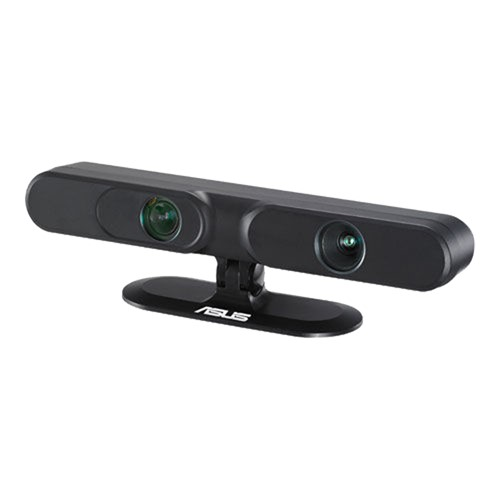
\includegraphics[width=0.5\textwidth]{figures/asus-xtion-pro.jpeg}
  \caption{The ASUS Xtion Pro is equipped with a depth sensor and it is 
      easily configurable to make it work with ROS. This simplifies the 
      integration with \texttt{elevation\_mapping} and, consequently, 
      the construction of a navigable map.}
  \label{fig:asus-xtion-pro}
\end{figure}

\section{World of Stairs}
(safe zone)
\begin{figure}
  \begin{subfigure}[b]{0.49\textwidth}
    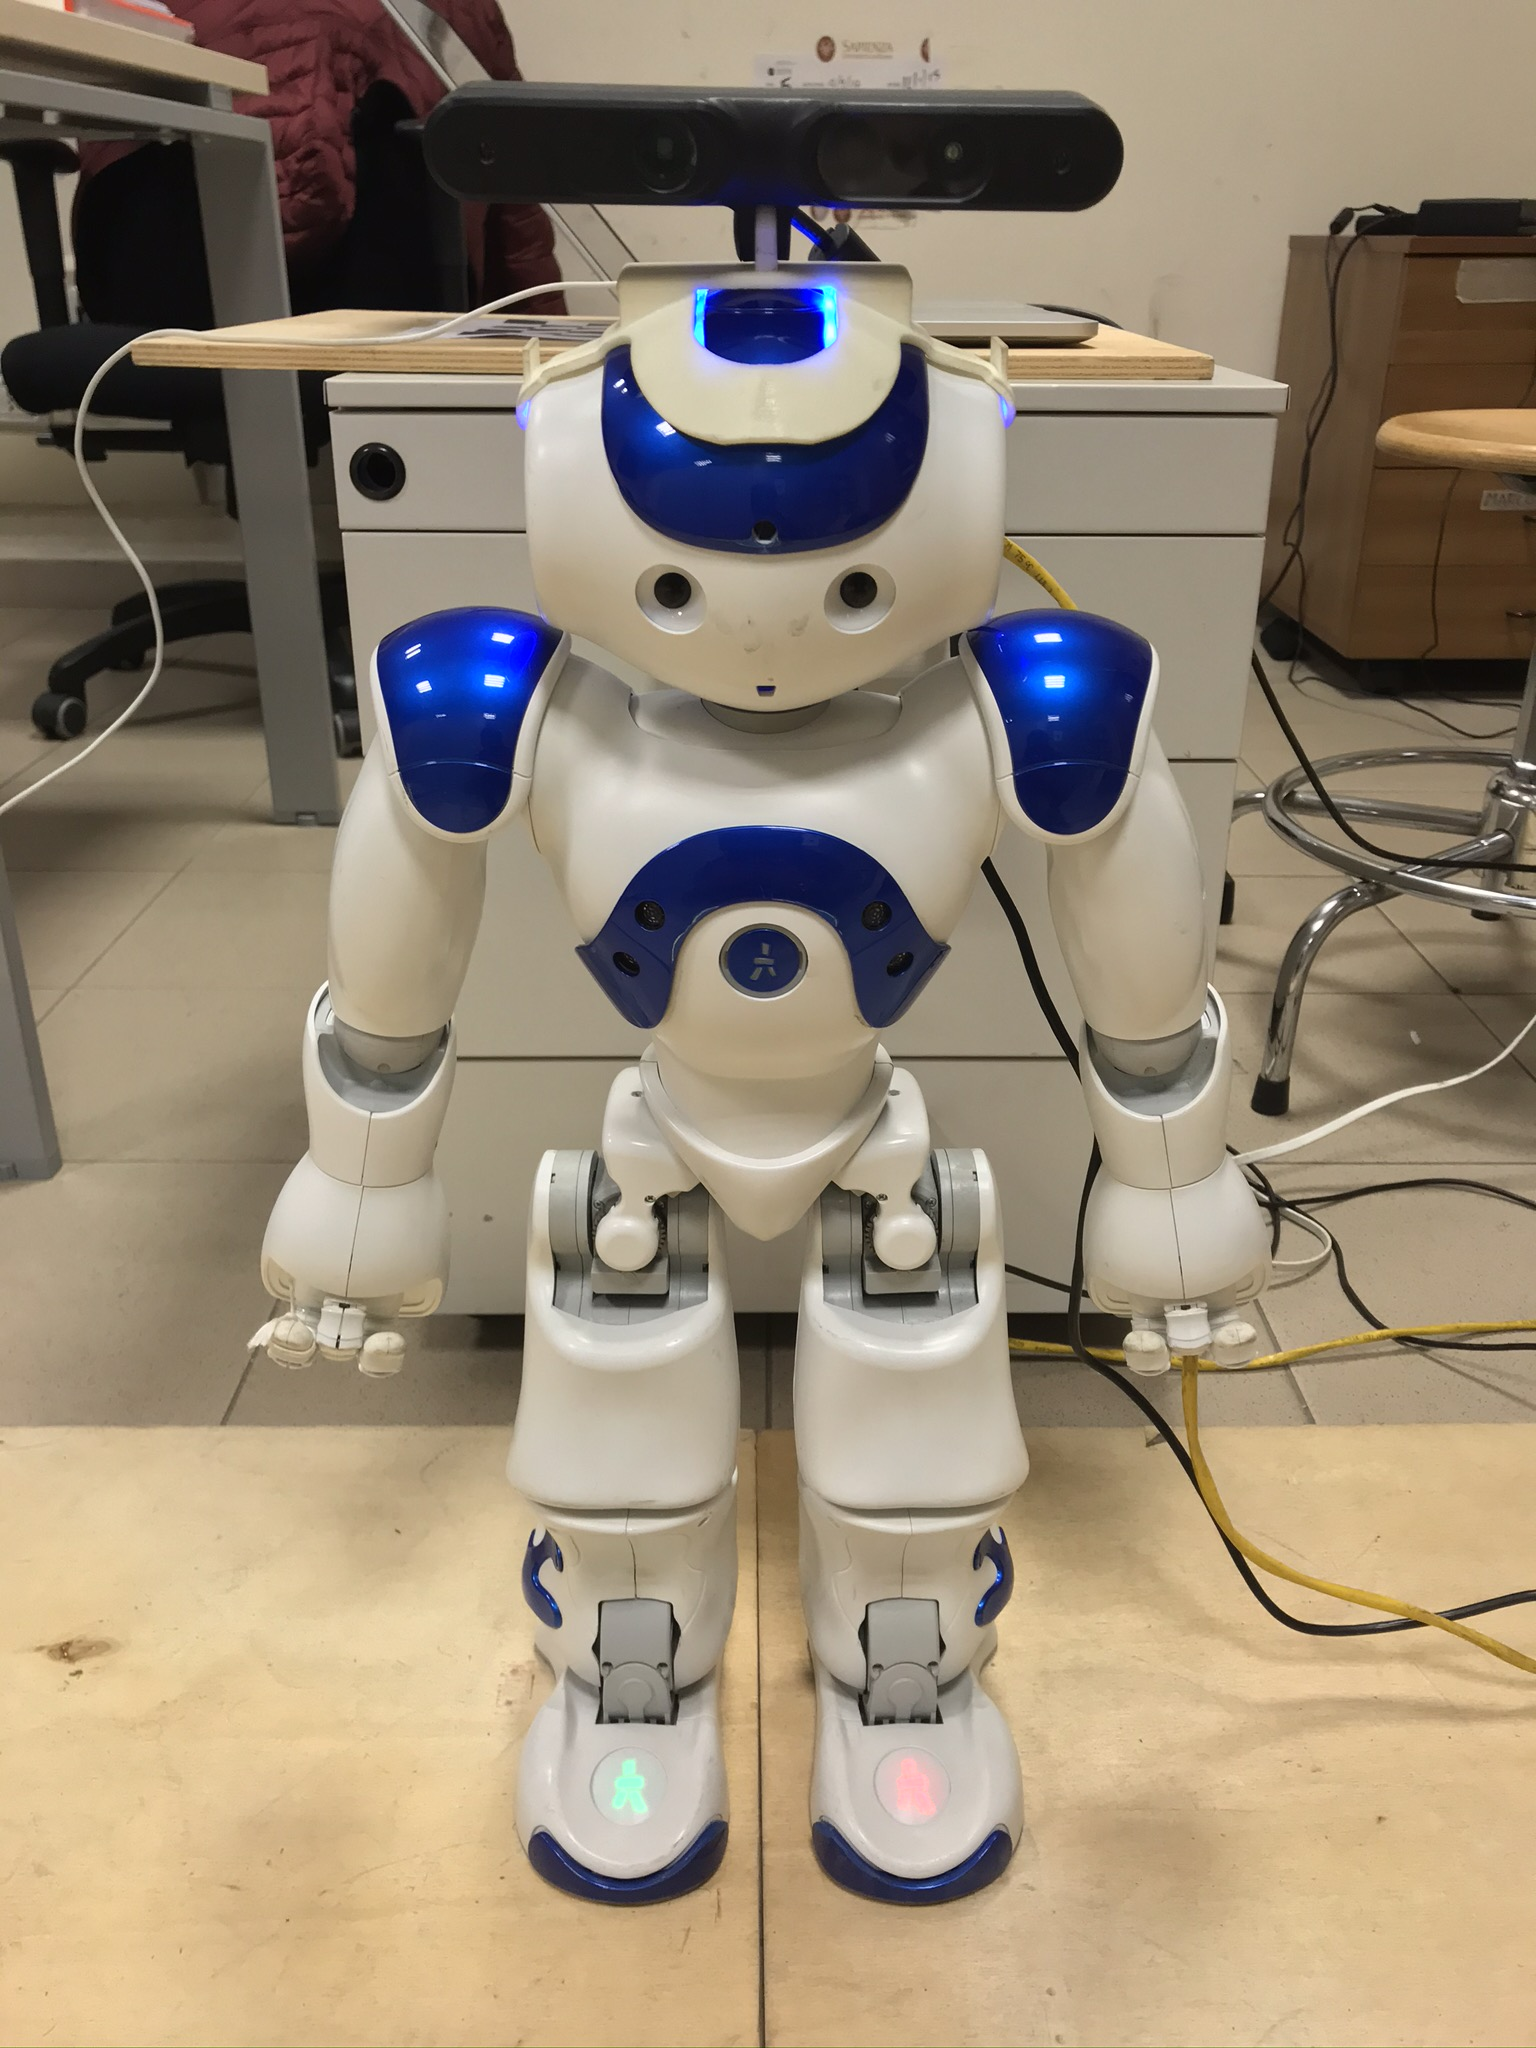
\includegraphics[width=\textwidth]{figures/NAO-with-xtion.JPEG}
    \caption{}
    \label{fig:nao-with-xtion}
  \end{subfigure}
  \hfill
  \begin{subfigure}[b]{0.49\textwidth}
    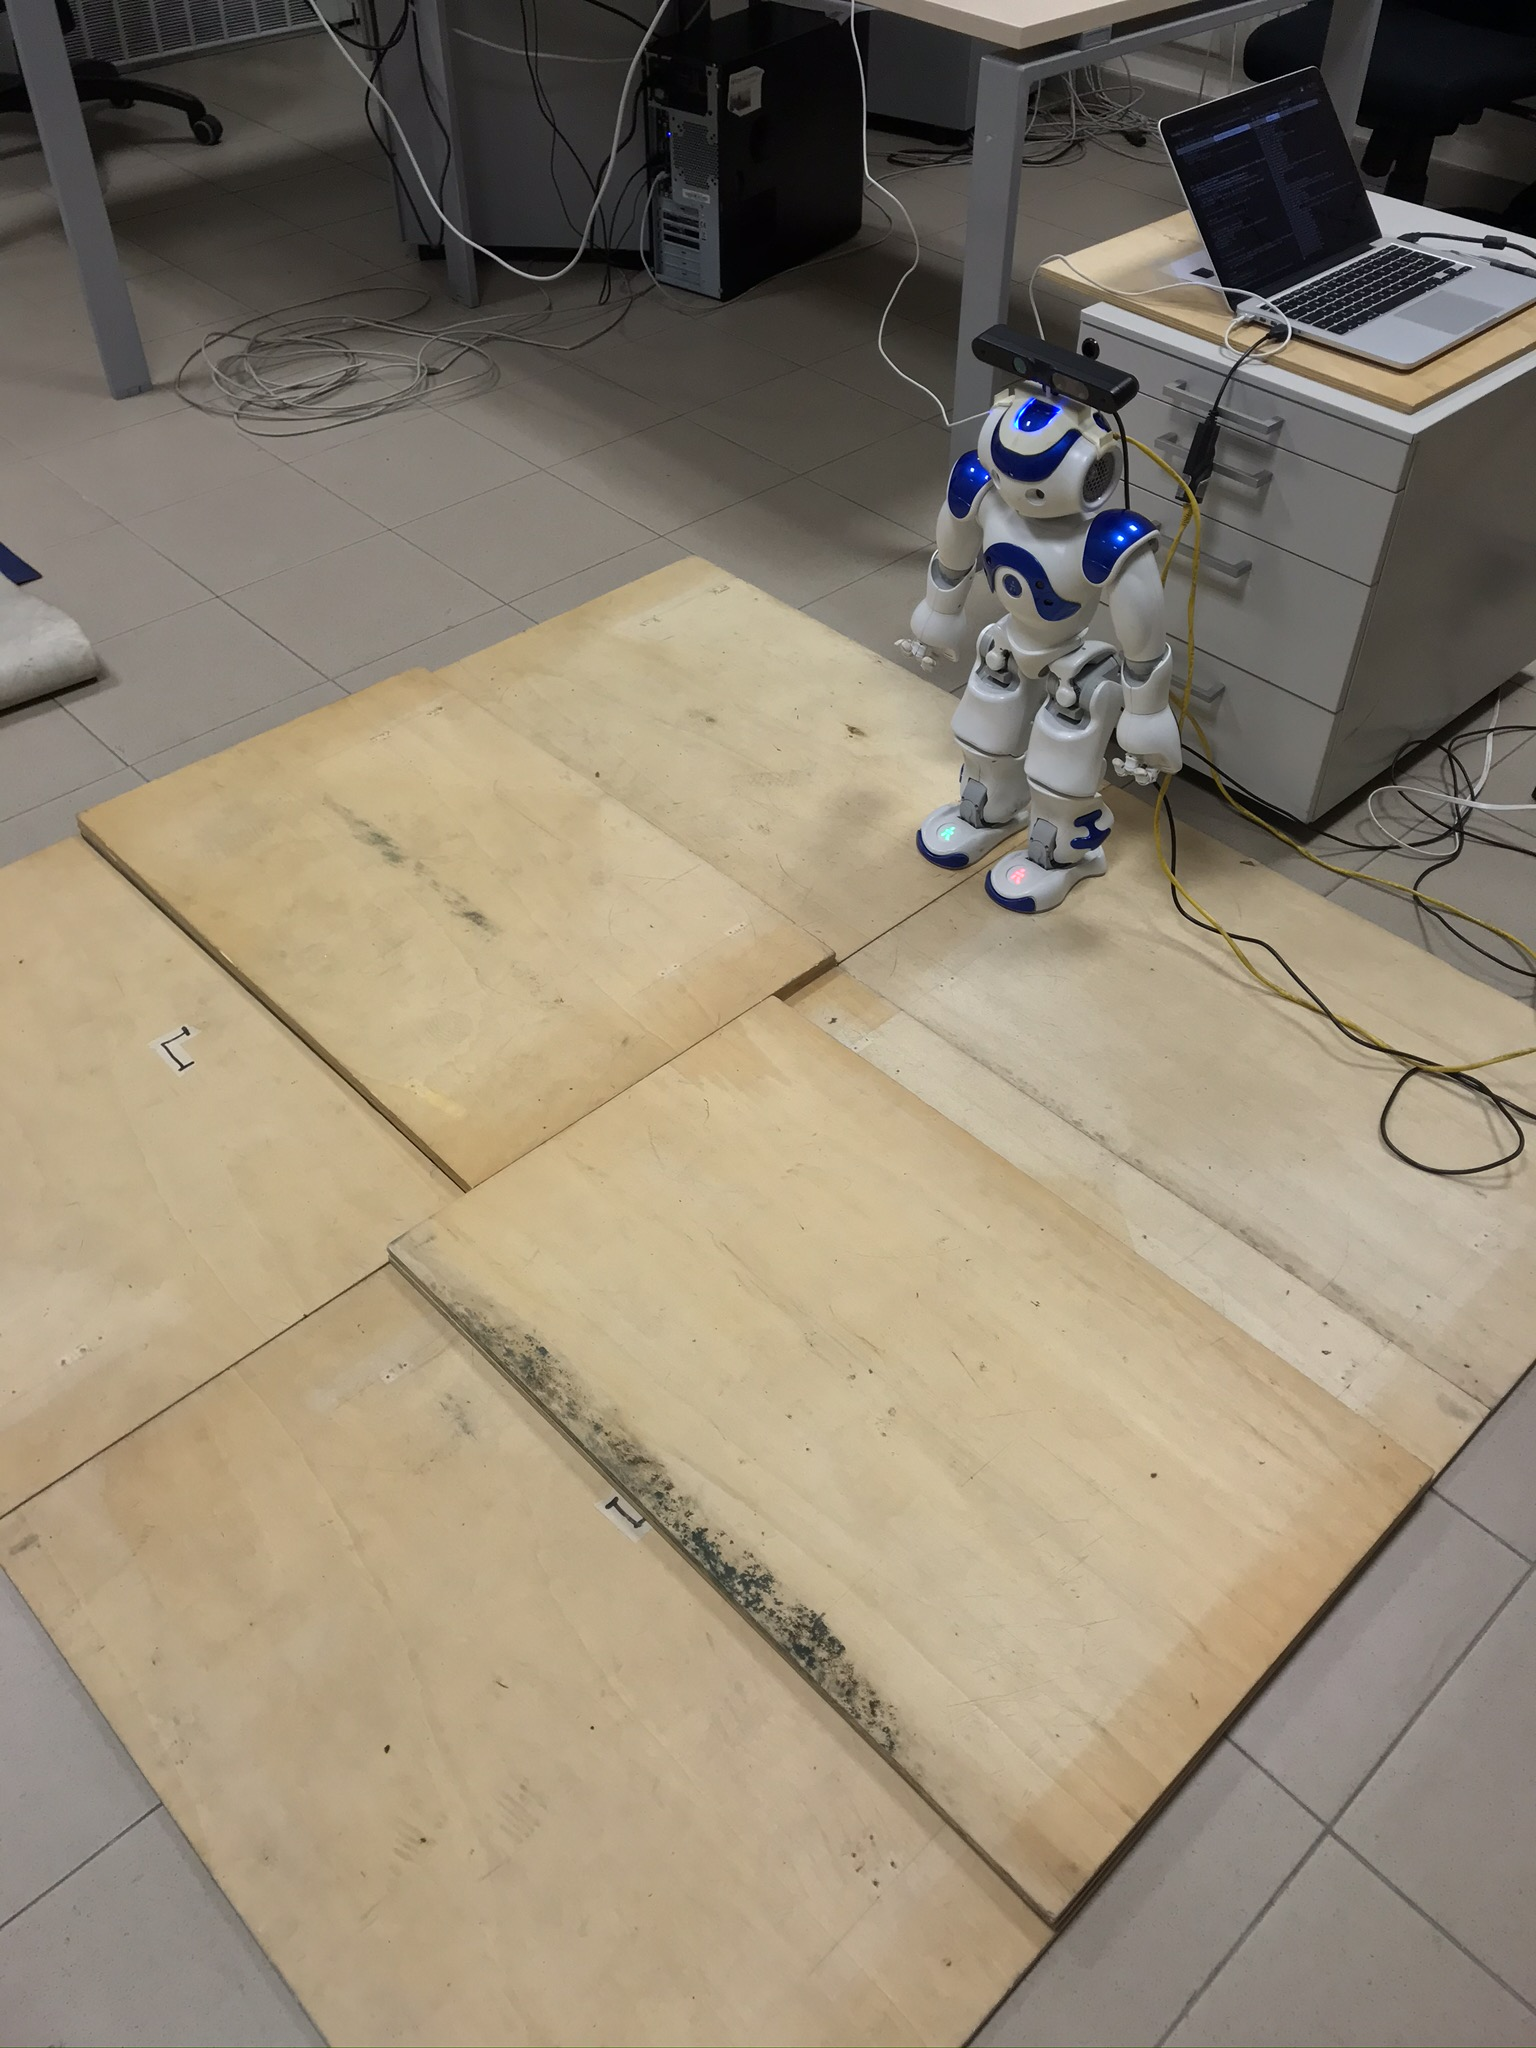
\includegraphics[width=\textwidth]{figures/NAO-with-xtion-full-env.JPEG}
    \caption{}
    \label{fig:nao-with-xtion-full-env}
  \end{subfigure}
  \caption{On the left, NAO humanoid robot with ASUS Xtion Pro placed on top.
      On the right, NAO humanoid robot in the environment described TODO, 
      right before starting the execution of the experiment.}
\end{figure}
\begin{figure}
  \centering
  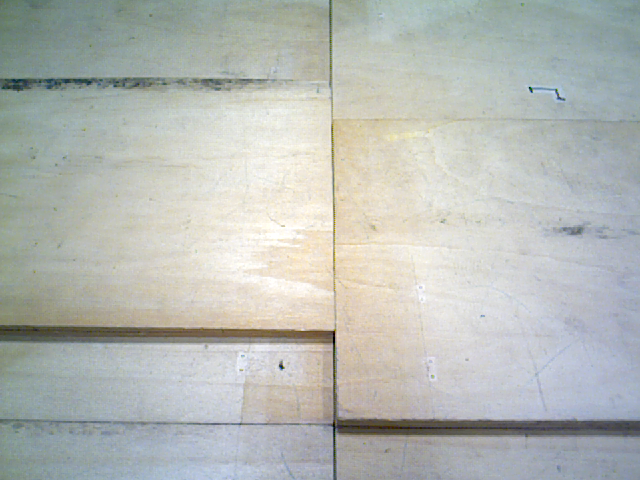
\includegraphics[width=0.85\textwidth]{figures/xtion_rgb_20cm.png}
  \caption{RGB image seen by the ASUS Xtion Pro placed on top of the robot.
      The corresponding depth image is sent to \texttt{elevation\_mapping}
      to build the map.}
  \label{fig:xtion-rgb-20cm}
\end{figure}
\begin{figure}
  \centering
  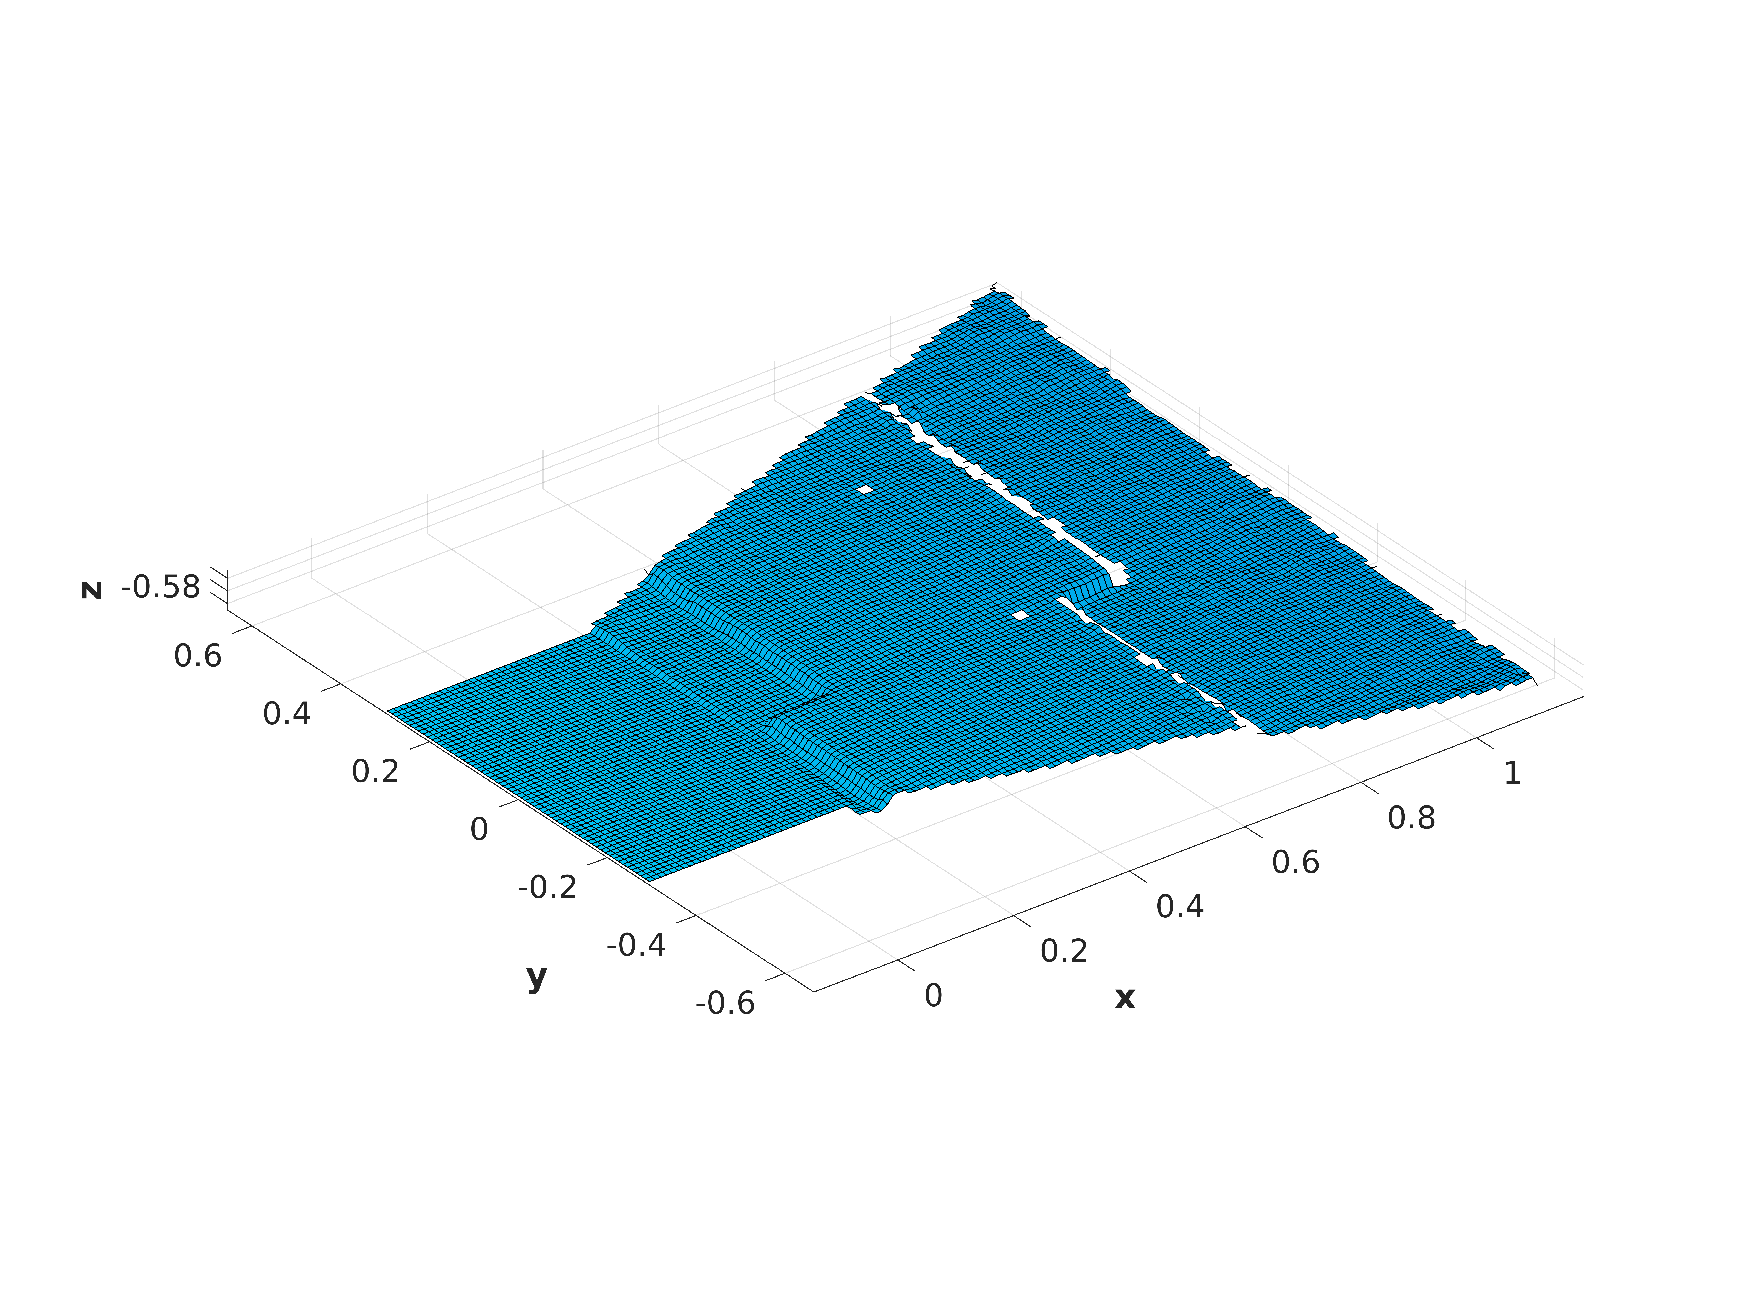
\includegraphics[width=\textwidth]{figures/onlymap-xtion-20cm.pdf}
  \caption{Elevation map build by \texttt{elevation\_mapping} for the 
      environment described TODO.}
  \label{fig:onlymap-xtion-20cm}
\end{figure}

